
%%%%%%%%%%%%%%%%%%%% file CSMC_MUME_LaTeX_Template.tex %%%%%%%%%%%%%%%%%%%%%
%
% This is the LaTeX source for the instructions to authors using
% the LaTeX document class 'llncs.cls' for contributions to
% the Journal of Creative Music Systems.
% Copyright: http://www.springer.com/lncs       Springer Heidelberg 2006/05/04
%
% It may be used as a template for your own input - copy it
% to a new file with a new name and use it as the basis
% for your article.
%
% NB: the document class 'llncs' has its own and detailed documentation, see
% ftp://ftp.springer.de/data/pubftp/pub/tex/latex/llncs/latex2e/llncsdoc.pdf
%
%%%%%%%%%%%%%%%%%%%%%%%%%%%%%%%%%%%%%%%%%%%%%%%%%%%%%%%%%%%%%%%%%%%

\documentclass[runningheads,a4paper]{llncs}

\usepackage{amssymb}
\setcounter{tocdepth}{3}
\usepackage{graphicx}
\usepackage{url}
\usepackage{apacite}
%added 
\usepackage[inline]{enumitem}    
\usepackage{subcaption}
\usepackage{caption}
\usepackage{threeparttable} %annotations for table
\usepackage{csquotes}


\newcommand{\keywords}[1]{\par\addvspace\baselineskip
\noindent\keywordname\enspace\ignorespaces#1}

\pagestyle{headings}

\begin{document}

\mainmatter  % start of an individual contribution

% first the title is needed
\title{Percussive Sound Generation with Virtual Listeners and Modular Synthesizers}

% a short form should be given in case it is too long for the running head
\titlerunning{Running Title}

% the name(s) of the author(s) follow(s) next
%
% NB: Chinese authors should write their first names(s) in front of
% their surnames. This ensures that the names appear correctly in
% the running heads and the author index.
%
\author{Amir Salimi \and Abram Hindle}
%
% if the names of the authors are too long for the running head, please use the format: AuthorA et al.
\authorrunning{Amir Salimi and Abram Hindle }

% the affiliations are given next; don't give your e-mail address
% unless you accept that it will be published
\institute{Department of Computing Science\\ University of Alberta \\ \email{asalimi@ualberta.ca}}

%
% NB: a more complex sample for affiliations and the mapping to the
% corresponding authors can be found in the file "llncs.dem"
% (search for the string "\mainmatter" where a contribution starts).
% "llncs.dem" accompanies the document class "llncs.cls".
%

\maketitle

\begin{abstract}
Digital sound artists often require a variety of percussive samples for their music. For more than two decades research involving digital synthesis, heuristic search, and neural networks has been used for the generation of novel sounds. Our goal is to generate one-shot percussive samples by leveraging modern AI technologies alongside scalable signal generation methods. We centered our approach around the combination of two central components: \begin {enumerate*} [label=(\roman*)] \item a \emph{virtual ear} capable of evaluating the proximity of unheard sounds to  and \item a dynamic \emph{virtual synthesizer} with a rich set of tractable parameters\end{enumerate*}. We present a generative pipeline that utilizes robust digital signal processing methods guided by supervised learning towards the generation of one-shot percussive sounds. We present our findings and measurements of the various approaches taken. Advantages, shortcomings and practicality of the employed methodologies are demonstrated. We share our curated dataset of sounds and codebase\footnote{\url{https://github.com/imilas/Synths_Stacks_Search}} which can be used for its further expansion.
\keywords{Automatic Synthesizer design. Machine Listening. Sound Analysis. Novelty and Originality}
\end{abstract}

\section{Introduction}

This is a \LaTeX{} template for submission to the \textit{2020 Joint Conference on AI Music Creativity (CSMC + MuMe)}.

\section{Paper Preparation}

When you use \LaTeX\ together with our document class file,
\texttt{llncs.cls},
your text is typeset automatically in Computer Modern Roman (CM) fonts.
Please do
\emph{not} change the preset fonts. If you have to use fonts other
than the preset fonts, kindly submit these with your files.

Please use the commands \verb+\label+ and \verb+\ref+ for
cross-references and the commands \verb+\bibitem+ and \verb+\cite+ for
references to the bibliography, to enable us to create hyperlinks at
these places.

For preparing your figures electronically and integrating them into
your source file we recommend using the standard \LaTeX{} \verb+graphics+ or
\verb+graphicx+ package. These provide the \verb+\includegraphics+ command.
In general, please refrain from using the \verb+\special+ command.

Remember to submit any further style files and
fonts you have used together with your source files.

\subsubsection{Headings.}

Headings should be capitalized
(i.e., nouns, verbs, and all other words
except articles, prepositions, and conjunctions should be set with an
initial capital) and should,
with the exception of the title, be aligned to the left.
Words joined by a hyphen are subject to a special rule. If the first
word can stand alone, the second word should be capitalized.

Here are some examples of headings: ``Criteria to Disprove
Context-Freeness of Collage Language'', ``On Correcting the Intrusion of
Tracing Non-deterministic Programs by Software'', ``A User-Friendly and
Extendable Data Distribution System'', ``Multi-flip Networks:
Parallelizing GenSAT'', ``Self-determinations of Man''.

\subsubsection{Lemmas, Propositions, and Theorems.}

The numbers accorded to lemmas, propositions, and theorems, etc. should
appear in consecutive order, starting with Lemma 1, and not, for
example, with Lemma 11.

\subsection{Figures}

For \LaTeX\ users, we recommend using the \emph{graphics} or \emph{graphicx}
package and the \verb+\includegraphics+ command.

Please check that the lines in line drawings are not
interrupted and are of a constant width. Grids and details within the
figures must be clearly legible and may not be written one on top of
the other. Line drawings should have a resolution of at least 800 dpi
(preferably 1200 dpi). The lettering in figures should have a height of
2~mm (10-point type). Figures should be numbered and should have a
caption which should always be positioned \emph{under} the figures, in
contrast to the caption belonging to a table, which should always appear
\emph{above} the table; this is simply achieved as matter of sequence in
your source.

Please centre the figures or your tabular material by using the \verb+\centering+
declaration. Short captions are centred by default between the margins
and typeset in 9-point type (Fig.~\ref{fig:example} shows an example).
The distance between text and figure is preset to be about 8~mm, the
distance between figure and caption about 6~mm.

To ensure that the reproduction of your illustrations is of a reasonable
quality, we advise against the use of shading. The contrast should be as
pronounced as possible.

If screenshots are necessary, please make sure that you are happy with
the print quality before you send the files.

\begin{figure}
	\centering
	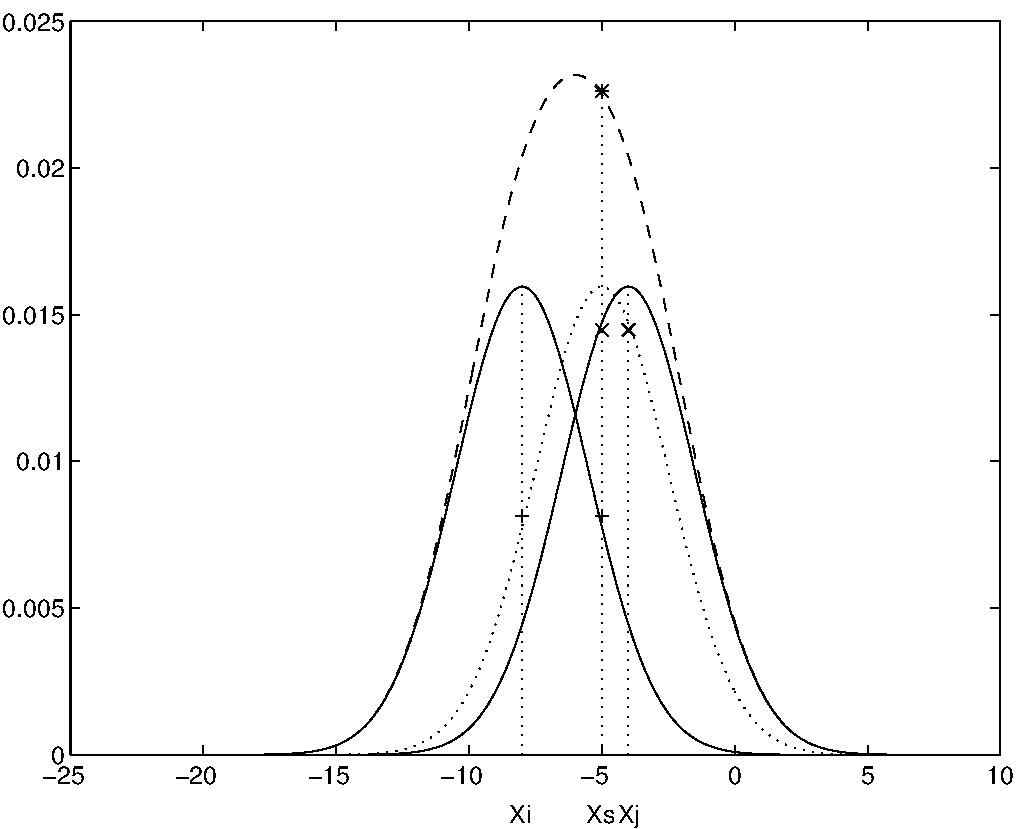
\includegraphics[height=6.2cm]{graphic.pdf}
	\caption{One kernel at $x_s$ (\emph{dotted kernel}) or two kernels at
	$x_i$ and $x_j$ (\textit{left and right}) lead to the same summed estimate
	at $x_s$. This shows a figure consisting of different types of
	lines. Elements of the figure described in the caption should be set in
	italics, in parentheses, as shown in this sample caption.}
	\label{fig:example}
\end{figure}

Please define figures (and tables) as floating objects. Please avoid
using optional location parameters like ``\verb+[h]+'' for ``here''.

\subsection{Formulas}

Displayed equations or formulas are centred and set on a separate
line (with an extra line or halfline space above and below). Displayed
expressions should be numbered for reference. The numbers should be
consecutive within each section or within the contribution,
with numbers enclosed in parentheses and set on the right margin --
which is the default if you use the \emph{equation} environment, e.g.,

\begin{equation}
  \psi (u) = \int_{o}^{T} \left[\frac{1}{2}
  \left(\Lambda_{o}^{-1} u,u\right) + N^{\ast} (-u)\right] dt \;  .
\end{equation}

Equations should be punctuated in the same way as ordinary
text but with a small space before the end punctuation mark.

\subsection{Footnotes}

The superscript numeral used to refer to a footnote appears in the text
either directly after the word to be discussed or -- in relation to a
phrase or a sentence -- following the punctuation sign (comma,
semicolon, or period). Footnotes should appear at the bottom of
the normal text area, with a line of about 2~cm set
immediately above them.\footnote{The footnote numeral is set flush left
and the text follows with the usual word spacing.}

\subsection{Program Code}

Program listings or program commands in the text are normally set in
typewriter font, e.g., CMTT10 or Courier.

\medskip

\noindent
{\it Example of a Computer Program}
\begin{verbatim}
program Inflation (Output)
  {Assuming annual inflation rates of 7%, 8%, and 10%,...
   years};
   const
     MaxYears = 10;
   var
     Year: 0..MaxYears;
     Factor1, Factor2, Factor3: Real;
   begin
     Year := 0;
     Factor1 := 1.0; Factor2 := 1.0; Factor3 := 1.0;
     WriteLn('Year  7% 8% 10%'); WriteLn;
     repeat
       Year := Year + 1;
       Factor1 := Factor1 * 1.07;
       Factor2 := Factor2 * 1.08;
       Factor3 := Factor3 * 1.10;
       WriteLn(Year:5,Factor1:7:3,Factor2:7:3,Factor3:7:3)
     until Year = MaxYears
end.
\end{verbatim}
%
\noindent
{\small (Example from Jensen K., Wirth N. (1991). \textit{Pascal user manual and
report}. New York: Springer)}

\subsection{Citations}

For citations in the text please use the APA6 system (\url{http://www.apastyle.org/}).

Examples:
\cite{einstein}
\cite<e.g.,>{knuthwebsite}
\cite[p.~10]{latexcompanion}
\citeA{latexcompanion}
(\citeNP{einstein}; \citeNP{latexcompanion})
\cite[pp.~10--11]{einstein}

\subsection{Page Numbering and Running Heads}

There is no need to include page numbers. If your paper title is too
long to serve as a running head, it will be shortened. Your suggestion
as to how to shorten it would be most welcome.

\subsubsection*{Acknowledgements} The heading should be treated as a
subsubsection heading and should not be assigned a number.

\section{The References Section}\label{references}

Please use the APA6 style for references.
The reference section must be complete. You may not omit references.
Instructions as to where to find a fuller version of the references are
not permissible.

We only accept references written using the Latin alphabet. If the title
of the book you are referring to is in Russian or Chinese, then please write
(in Russian) or (in Chinese) at the end of the transcript or translation
of the title.

The following section shows a sample reference list.

\bibliographystyle{apacite}
% Place your own .bib file here:
\bibliography{CSMC_MUME_LaTeX_Template.bib}

\end{document}
